
C++20对现有的并发性进行了增强,但我们将重点关注新添加的特性:协程。协程具有中断和恢复功能的线程,在几种主要的应用程序中很有用:可以极大地简化事件驱动程序的编写,对于窃取工作的线程池来说,那必然要使用协程,而且会让异步I/O和其他异步的代码更加简单

\subsubsubsection{8.4.1\hspace{0.2cm}介绍协程}

协同程序有两种风格:\textbf{有栈}和\textbf{无栈}。有栈协程有时也被称为\textbf{纤程}(fiber),类似于在堆栈上分配状态的函数。无栈协程没有相应的堆栈,状态存储在堆中。通常,有栈协程更加强大和灵活,但是无栈协程会更高效。

本书中,我们将重点关注无栈协程,因为C++20支持。这是一个不寻常的概念,在展示C++特有的语法和示例之前,先来解释一下。

常规的C++函数总是有一个相应的堆栈框架。只要函数在运行,栈帧就存在,所有的局部变量和其他状态都存储在这里。下面是一个简单的函数\texttt{f()}:

\begin{lstlisting}[style=styleCXX]
void f() {
	…
}
\end{lstlisting}

其中有一个栈帧。再函数\texttt{f()}调用另一个函数\texttt{g()}时:

\begin{lstlisting}[style=styleCXX]
void g() {
	…
}
void f() {
	…
	g();
	…
}
\end{lstlisting}

函数\texttt{g()}在函数运行时也有一个栈帧。 

参考下图:

%\hspace*{\fill} \\ %插入空行
\begin{center}
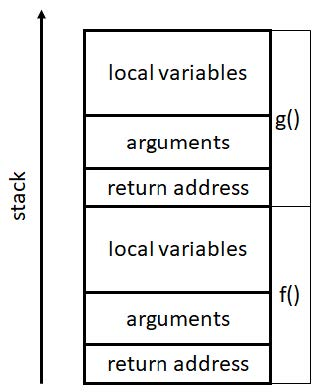
\includegraphics[width=0.6\textwidth]{content/2/chapter8/images/5.jpg}\\
图8.5 - 常规函数的栈帧
\end{center}

当函数\texttt{g()}退出时,它的栈帧会销毁,只有函数\texttt{f()}的栈帧保留了下来。

相反,无栈协程的状存储在堆上:这种分配称为\textbf{活帧}。活帧与协程句柄相关联,协程句柄是一个智能指针的对象。可以发出和返回函数的调用,只要句柄没有损坏,活帧就一直存在。

协程还需要堆栈空间,比如调用其他函数。该空间在调用者的堆栈上分配。下面是它的工作原理(C++语法有所不同,所以现在把协程相关的行为想象成伪代码):

\begin{lstlisting}[style=styleCXX]
void g() {
	…
}
void coro() { // coroutine
	…
	g();
	…
}
void f() {
	…
	std::coroutine_handle<???> H; // Not the real syntax
	coro();
	…
}
\end{lstlisting}

对应的内存分配如下图所示:

%\hspace*{\fill} \\ %插入空行
\begin{center}
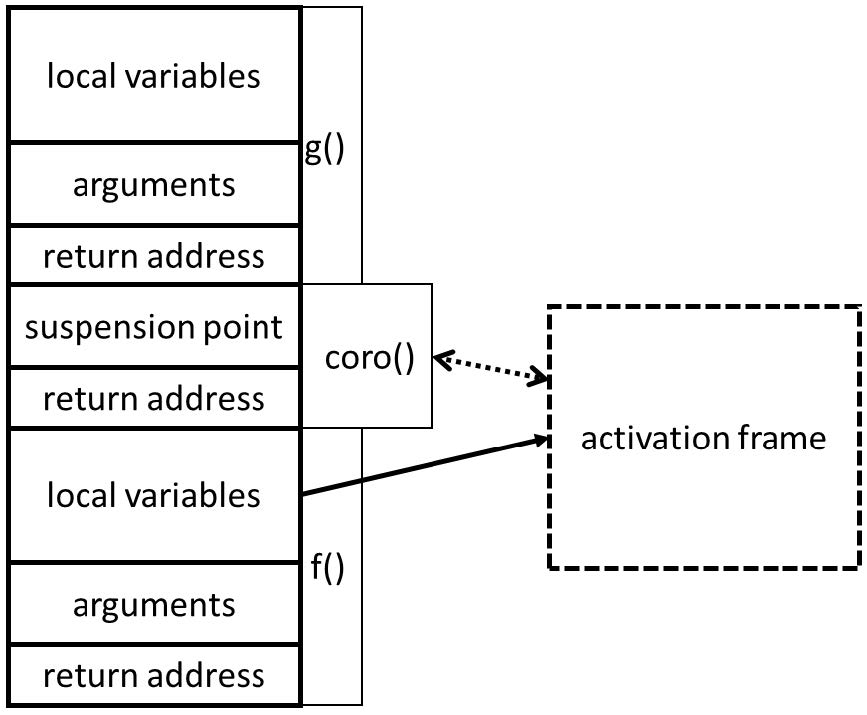
\includegraphics[width=0.6\textwidth]{content/2/chapter8/images/6.jpg}\\
图8.6 - 调用协程
\end{center}

函数\texttt{f()}创建协程句柄,所以拥有活帧。然后调用协程函数\texttt{coro()}。这时有一些堆栈分配,协程在堆栈上存储了在挂起时返回的地址(记住,协程是可以挂起自己的函数)。协程可以调用另一个函数\texttt{g()},将\texttt{g()}的栈帧分配到堆栈上。此时,协程不能再挂起:只有协程顶层函数可以挂起。函数\texttt{g()}无论谁调用最终都会返回,以同样的方式运行,这将破坏它的栈帧。协程现在可以挂起自己了,所以我们假设它挂起了。 

这是有栈协程和无栈协程的关键区别:有栈协程可以在函数调用任意深度的地方挂起,并将从那里恢复。但是这种灵活性需要很高的内存成本,尤其是运行时成本:无栈协程由于其有限的状态,效率要高很多。

当协程挂起时,恢复协程所需的部分状态会存储在活帧中。然后销毁协程的栈帧,并将控制权返回给调用者,直至协程调用的位置。如果协程完成,也会发生同样的情况,但是调用者有一种方法可以查询协程的状态是挂起还是完成。

调用者继续执行他的操作,并可以使用其他函数:

\begin{lstlisting}[style=styleCXX]
void h() {
	…
}
void coro() {…} // coroutine
void f() {
	…
	std::coroutine_handle<???> H; // Not the real syntax
	coro();
	h(); // Called after coro() is suspended
	…
}
\end{lstlisting}

内存分配看起来如下所示:

%\hspace*{\fill} \\ %插入空行
\begin{center}
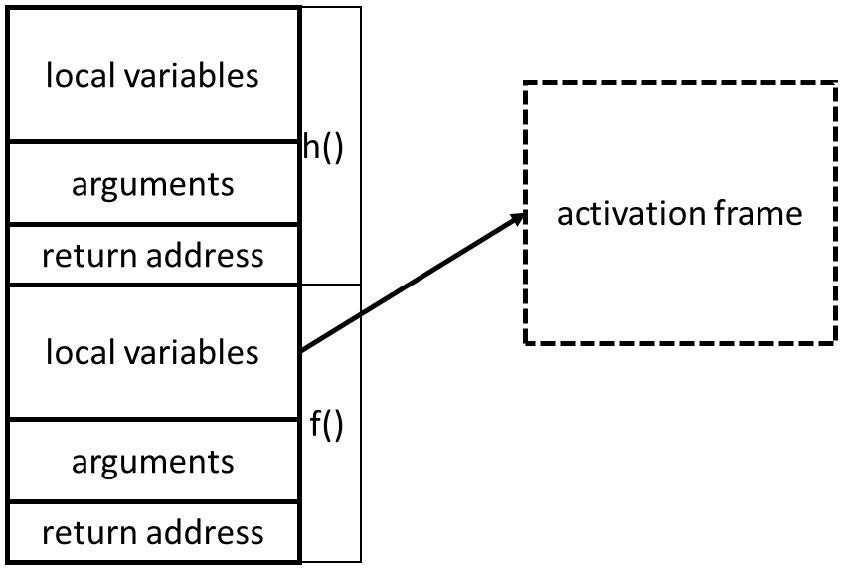
\includegraphics[width=0.6\textwidth]{content/2/chapter8/images/7.jpg}\\
图8.7 - 挂起协程,继续执行
\end{center}

注意,没有与协程对应的栈帧,只有堆分配的活帧。只要句柄对象处于活动状态,协程就可以恢复。不一定是调用和恢复协程的同一函数,例如:如果句柄可用,函数\texttt{h()}就可以恢复:

\begin{lstlisting}[style=styleCXX]
void h(H) {
	H.resume(); // Not the real syntax
}
void coro() {…} // coroutine
void f() {
	…
	std::coroutine_handle<???> H; // Not the real syntax
	coro();
	 h(H); // Called after coro() is suspended
	…
}
\end{lstlisting}

协程从暂停的地方重新开始,状态从活帧中恢复,任何必要的堆栈分配将像往常一样:

%\hspace*{\fill} \\ %插入空行
\begin{center}
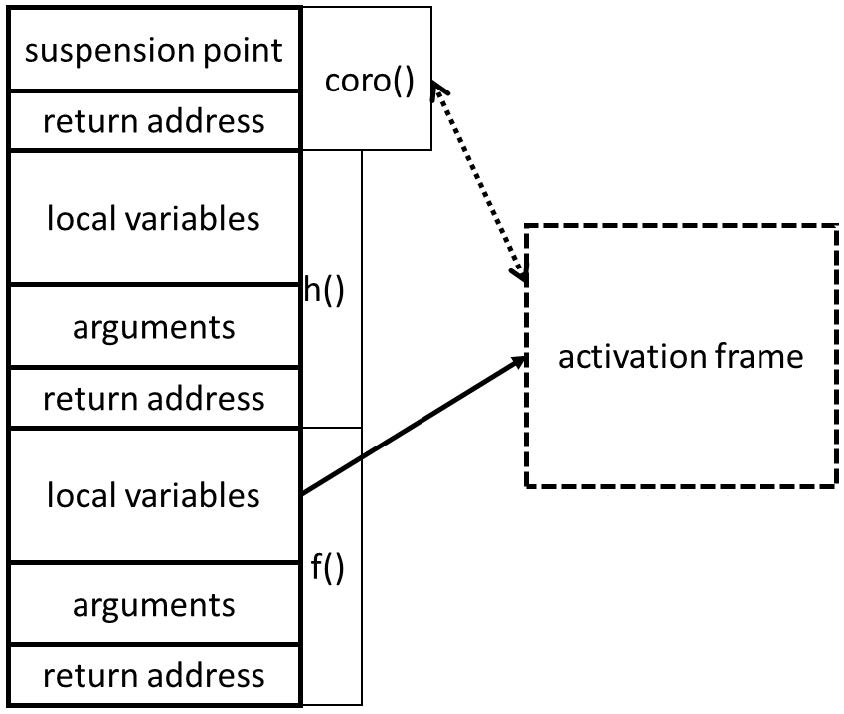
\includegraphics[width=0.6\textwidth]{content/2/chapter8/images/8.jpg}\\
图8.8 - 协程从不同的函数处恢复
\end{center}.

最终,协程完成,句柄销毁。这将释放与协程关联的所有内存。

以下是关于C++20协程需要了解的主要内容:

\begin{itemize}
\item
协程是可以挂起自己的函数。这与操作系统挂起一个线程不同:挂起一个协程是由开发者显式地完成的(多任务协作)。

\item
与栈帧相关联的常规函数不同,协程具有句柄对象。只要句柄处于活动状态,协程状态就会保持。

\item
协程挂起后,控制权将返回给调用者,调用者可以继续以相同的方式运行,就像协程已经完成一样。 

\item 
协程可以从任何位置恢复,不一定是调用者本身。此外,协程甚至可以从不同的线程恢复(将在本节后面看到一个示例)。协程从挂起点恢复,并继续运行,就像什么都没发生一样(但可能在不同的线程上运行)。
\end{itemize}

现在让我们了解一下所有这些在C++中是如何完成的。

\subsubsubsection{8.4.2\hspace{0.2cm}协程的C++语法}

现在让我们看一下C++语言的构造,这些构造可用于协程编程。 

首先,是获得一个支持该特性的编译器。GCC和Clang在他们的最新版本中都支持协程,但不幸的是,方式不同。对于GCC您需要版本11或更高版本。对于Clang,在版本10中添加了部分支持,并在以后的版本中进行了加强,但仍然是“实验性的”。

首先,为了编译协程代码,您需要在命令行上有一个编译器选项(使用\texttt{-std=c++20}选项启用C++20还不够)。对于GCC,这个选项是\texttt{-fcoroutines}。对于Clang,选项是\texttt{-stdlib=libc++ -fcoroutines-ts}。最新版的Visual Studio只需要\texttt{/std:c++20},不需要其他选项。

然后,需要包含协程头文件。在GCC和Visual Studio中(根据标准),头文件是\texttt{\#include <coroutine>},声明的所有类都在标准命名空间\texttt{std}中。但在Clang中,头文件是\texttt{\#include <experimental/coroutine>},使用的命名空间是\texttt{std::experimental}。

声明协程不需要特殊的语法,协程只是普通的C++函数。使它们成为协程的是使用暂停操作\texttt{co\_await}或其\texttt{co\_yield}。然而,在函数体中调用这些操作是不够的,C++中的协程对其返回类型有严格的要求。标准库在声明这些返回类型和其他处理协程所需的类时,没有提供任何帮助。语言仅提供了一个使用协程进行编程的框架。因此,直接使用C++20协程代码会非常冗长、重复,并且包含大量样板代码。实际中,每个使用协程的开发者都会使用一个可用的协程库。 

对于实际的编程,也应该这样做。本书中,我们将展示用简单的C++编写的示例。这样做的目的是,不想引入任何特定的库,而且这样做会模糊读者对实际情况的理解。对协程的支持是最近才出现的,这些库也在迅速发展,现在选择的库不一定会一直好用。我们希望在C++的级别理解协程代码,而不是在某个特定库所呈现的抽象级别理解协程代码。然后,应该根据自己的需要选择一个库,并使用它的抽象语法进行编程。

对与协程相关语法结构的全面描述非常不直观:它是一个框架,而不是一个库。出于这个原因,我们将使用示例来完成余下的演示。如果真的想知道协程的所有语法要求,必须查找最新的出版物(或阅读标准)进行了解。但是这些例子应该能对协程的功能有足够的展示,也可以阅读相关协程库的文档,并在程序中使用这个协程库。

\subsubsubsection{8.4.3\hspace{0.2cm}协程用例}

第一个例子是C++中协程最常见的用法(标准为协程提供了一些显式设计的语法)。我们将实现一个惰性生成器。生成器是生成数据序列的函数。每次调用生成器,都会得到序列的一个新元素。惰性生成器是按需计算元素的生成器。

下面是一个基于C++20协程的惰性生成器:

\hspace*{\fill} \\ %插入空行
\noindent
\textbf{coroutines\_generator1.C}
\begin{lstlisting}[style=styleCXX]
generator<int> coro(){
	for (int i = 0;; ++i) {
		co_yield i;
	}
}
int main() {
	auto h = coro().h_;
	auto& promise = h.promise();
	for (int i = 0; i < 3; ++i) {
		std::cout << "counter: " << promise.value_ << 
		std::endl;
		h();
	}
	h.destroy();
}
\end{lstlisting}

As promised, this is very low-level C++, you rarely see code like this, but it allows us to explain all the steps. First of all, the coroutine coro() looks like any other function, except for the co\_yield operator. This operator suspends the coroutine and returns the value i to the caller. Because the coroutine is suspended, not terminated, the operator can be executed multiple times. Just like any other function, the coroutine terminates when the control reaches the closing brace; at this point, it cannot be resumed. It is possible to exit the coroutine at any point by executing statement co\_return (the regular return statement should not be used).

Second, the return type of the coroutine – generator – is a special type that we are about to define. It has a lot of requirements on it, which results in lengthy boilerplate code (any coroutine library will have such types predefined for you). We can already see that generator contains a nested data member h\_; that is the coroutine handle. The creation of this handle also creates the activation frame. The handle is associated with a promiseobject; this has absolutely nothing to do with C++11 std::promise. In fact, it is not one of the standard types at all: we have to define it according to a set of rules listed in the standard. At the end of the execution, the handle is destroyed, which destroys the coroutine state as well. The handle is, thus, similar to a pointer.

Finally, the handle is a callable object. Calling it resumes the coroutine, which generates the next value and promptly suspends itself again because the co\_yield operator is in the loop. 

All of this is magically tied together by defining the appropriate return type for the coroutine. Just like the STL algorithms, the entire system is bound by convention: there are expectations on all types involved in this process, and something somewhere will not compile if these expectations are not met. Let us see the generator type now:

\begin{lstlisting}[style=styleCXX]
template <typename T> struct generator {
	struct promise_type {
		T value_ = -1;
		generator get_return_object() {
			using handle= std::coroutine_handle<promise_type>;
			return generator{handle::from_promise(*this)};
		}
		std::suspend_never initial_suspend() { return {}; }
		std::suspend_never final_suspend() noexcept { return 
			{}; }
		void unhandled_exception() {}
		std::suspend_always yield_value(T value) {
			value_ = value;
			return {};
		}
	};
	std::coroutine_handle<promise_type> h_;
};
\end{lstlisting}

First of all, the return type does not have to be generated from a template. We could have just declared a generator for integers. Usually, it is a template parameterized on the type of the elements in the generated sequence. Second, the name generator is in no way special: you can call this type anything you want (most libraries provide a similar template and call it generator). On the other hand, the nested type generator::promise\_type must be called promise\_type, otherwise, the program will not compile. Often,  the nested type itself is called something else, and a type alias is used:

\begin{lstlisting}[style=styleCXX]
template <typename T> struct generator {
	struct promise { … };
	using promise_type = promise;
};
\end{lstlisting}

The promise\_type type must be a nested type of the generator class (or, in general, any type returned by the coroutine). But the promise class does not have to be a nested class: usually, it is, but it could be declared outside as well. 

What is mandatory is the set of required member functions of the promise type, including their signatures. Note that some of the member functions are declared noexcept. This is part of the requirement, too: the program will not compile if you omit this specification. Of course, any function that is not required to be noexcept can be declared as such if it doesn't throw. 

The body of these required functions may be more complex for different generators. We will describe briefly what each of them does.

The first non-empty function, get\_return\_object(), is part of the boilerplate code and usually looks exactly like the one earlier; this function constructs a new generator from a handle that is, in turn, constructed from a promise object. It is called by the compiler to get the result of the coroutine. 

The second non-empty function, yield\_value(), is invoked every time the operator co\_yield is called; its argument is the co\_yield value. Storing the value in the promise object is how the coroutine usually passes the results to the caller. 

The initial\_suspend() function is called by the compiler the first time co\_yield is encountered. The final\_suspend() function is called after the coroutine produces its last result via co\_return; it cannot be suspended afterward. If the coroutine ends without co\_return, the return\_void() method is called. Finally, if the coroutine throws an exception that escapes from its body, the unhandled\_exception() method is called. You can customize these methods for special handling of each of these situations, although this is seldom used.

Now we see how it all ties together to provide us with a lazy generator. First, the coroutine handle is created. In our example, we do not keep the generator object, only the handle. This is not required: we could have kept the generator object and destroyed the handle in its destructor. The coroutine runs until it hits co\_yield and suspends itself; the control is returned by the caller while the return value of co\_yield is captured in the promise. The calling program retrieves this value and resumes the coroutine by invoking the handle. The coroutine picks up from the point where it was suspended and runs until the next co\_yield. 

Our generator can run forever (or until we reach the maximum integer value on our platform, anyway): the sequence never ends. If we needed a sequence of finite length, we can execute co\_return or just exit the loop after the sequence is over. Refer to the following code:

\begin{lstlisting}[style=styleCXX]
generator<int> coro(){
	for (int i = 0; i < 10; ++i) {
		co_yield i;
	}
}
\end{lstlisting}

Now we have a sequence of 10 elements. The caller must check the result of the handle member function done() before trying to resume the coroutine.

We mentioned before that a coroutine can be resumed from anywhere in the code (after it was suspended, of course). It can even be resumed from a different thread. In this case, the coroutine starts to execute on one thread, is suspended, and then runs the rest of its code on another thread. Let us see an example:

\hspace*{\fill} \\ %插入空行
\noindent
\textbf{coroutines\_change\_threads.C}
\begin{lstlisting}[style=styleCXX]
task coro(std::jthread& t) {
	std::cout << "Coroutine started on thread: " <<
		std::this_thread::get_id() << '\n';
	co_await awaitable{t};
    std::cout << "Coroutine resumed on thread: " <<
		std::this_thread::get_id() << '\n';
	std::cout << "Coroutine done on thread: " <<
		std::this_thread::get_id() << '\n';
}
int main() {
	std::cout << "Main thread: " <<
		std::this_thread::get_id() << '\n';
	std::jthread t;
	coro(t);
	std::cout << "Main thread done: " << 
		std::this_thread::get_id() << std::endl;
}
\end{lstlisting}

First, let us get one detail out of the way: std::jthread is a C++20 addition, it is just a joinable thread – it is joined in the destructor of the object (almost anyone who worked with threads wrote a class for that, but now we have a standard one). Now we can move to the important part – the coroutine itself. 

First, let us see the return type of the coroutine:

\begin{lstlisting}[style=styleCXX]
struct task{
	struct promise_type {
		task get_return_object() { return {}; }
		std::suspend_never initial_suspend() { return {}; }
		std::suspend_never final_suspend() noexcept { return 
			{}; }
		void return_void() {}
		void unhandled_exception() {}
	};
};
\end{lstlisting}

This is actually the smallest possible return type of a coroutine: it contains all the required boilerplate and nothing else. Specifically, the return type is a class that defines a nested type promise\_type. That nested type must define several member functions, as shown in this code. Our generator type from the previous example has all of that plus some data used to return the results to the caller. Of course, the task can also have an internal state as needed.

The second change from the previous example is the way the task is suspended: we do it with co\_await instead of co\_yield. Operator co\_await is actually the most general way to suspend a coroutine: just like co\_yield, it suspends the function and returns the control to the caller. The difference is in the argument type: while co\_yield returns a result, co\_await's argument is an awaiter object with very general functionality. There are, again, specific requirements on the type of this object. If the requirements are met, the class is called an awaitable, and an object of this type is a valid awaiter (if not, something somewhere will not compile). Here is our awaitable:

\begin{lstlisting}[style=styleCXX]
struct awaitable {
	std::jthread& t;
	bool await_ready() { return false; }
	void await_suspend(std::coroutine_handle<> h) {
		std::jthread& out = t;
		out = std::jthread([h] { h.resume(); });
	}
	void await_resume() {}
	~awaitable() {}
	awaitable(std::jthread& t) : t(t) {}
};
\end{lstlisting}

The required interface of an awaitable is the three methods we see here. The first is await\_ready(): it is called after the coroutine is suspended. If it returns true, then the result of the coroutine is ready, and it is not really necessary to suspend it. In practice, it almost always returns false, which leads to suspension of the coroutine: the state of the coroutine, such as local variables and the suspension point, is stored in the activation frame, and the control is returned to the caller or resumer. The second function is await\_resume(), it is called just before the coroutine continues to execute after it is resumed. If it returns the result, that is the result of the entire co\_await operator (no result in our example). The most interesting function is await\_suspend(). It is called with the handle of the current coroutine when this coroutine is suspended and can have several different return types and values. If it returns void, as it does in our example, the coroutine is suspended, and the control is returned to the caller or resumer. Don't be fooled by the content of await\_suspend() in our example: it does not resume the coroutine. Instead, it creates a new thread that will execute a callable object, and it is this object that resumes the coroutine. The coroutine may be resumed after await\_suspend() is done or while it is still running: this example demonstrates the use of coroutines for asynchronous operations. 

Putting all of this together, we get this sequence:

\begin{enumerate}
\item
The main thread calls a coroutine.

\item
The coroutine is suspended by operator co\_await. This process involves several calls to the member functions of the awaitable object, one of which creates a new thread whose payload resumes the coroutine (the game with move-assigning thread objects is done so we delete the new thread in the main program and avoid some nasty race conditions).

\item
Control is returned to the caller of the coroutine, so the main thread continues to run from the line after the coroutine call. It will block in the destructor of the thread object t if it gets there before the coroutine completes.

\item 
The coroutine is resumed by the new thread and continues to execute on that thread from the line after co\_await. The awaitable object that was constructed by co\_await is destroyed. The coroutine runs to the end, all on the second thread. Reaching the end of the coroutine means it's done, just like any other function. The thread that runs the coroutine now can be joined. If the main thread was waiting for the destructor of thread t to complete, it now unblocks and joins the thread (if the main thread has not yet reached the destructor, it won't block when it does). 
\end{enumerate}

The sequence is confirmed by the output of our program:

\begin{tcblisting}{commandshell={}}
Main thread: 140003570591552
Coroutine started on thread: 140003570591552
Main thread done: 140003570591552
Coroutine resumed on thread: 140003570587392
Coroutine done on thread: 140003570587392
\end{tcblisting}

As you can see, the coroutine coro() was running on one thread first, then changed to a different thread in the middle of the execution. If it had any local variables, they would be preserved through this transition.

We mentioned that co\_await is the general operator for suspending coroutines. Indeed, the co\_yield x operator is equivalent to a particular invocation of co\_await as shown here:

\begin{lstlisting}[style=styleCXX]
co_await promise.yield_value(x);
\end{lstlisting}

Here promise is the promise\_type object associated with the current coroutine handle. The reason for the separate operator co\_yield is that accessing your own promise from inside the coroutine results in a quite verbose syntax, so the standard added a shortcut.

These examples demonstrate the capabilities of coroutines in C++. The situations where coroutines are thought to be useful are work stealing (you have seen how easy it is to transfer execution of a coroutine to another thread), lazy generators, and asynchronous operations (I/O and event handling). Nonetheless, the C++ coroutines have not been around long enough for any patterns to emerge, so the community is yet to come up with the best practices for using coroutines. Similarly, it is too early to talk about the performance of the coroutines; we have to wait for the compiler support to mature and for larger-scale applications to be developed. 

Overall, after neglecting concurrency for years, the C++ standard is rapidly catching up, so let us summarise the recent advances.









